\documentclass{scrartcl}

\usepackage{amsmath, amssymb, amsthm}
\usepackage{graphicx}
\usepackage{booktabs}
\usepackage{diagbox}

\newtheorem{example}{Example}

\title{Decibel}
\subtitle{A Dice Mechanic for Tabletop Role Playing Games}

\author{Michael Purcell}
\date{}

\begin{document}
\maketitle

\section{Simple Checks}\label{section:simple_checks}
To make a simple check, players roll a pool of three or more twenty-sided dice (d20s).  The outcome of the check is the difference between the largest and smallest values. We will write $N$dB to denote the outcome of a simple check made with a pool of $N$ twenty-sided dice.

\begin{example}
Suppose that a player is making a simple 5dB check.  The player rolls five twenty-sided dice and gets a result of $\{6,14,3,7,10\}$.  The outcome of the check is $14-3 = 11$.
\end{example}

Notice that while the set of possible outcomes (i.e. $\{0,1,\ldots,19$\}) is always the same, the size of the pool determines the distribution of the outcome of a check.  In general, larger dice pools are more likely to produce greater outcomes than smaller dice pools.

\section{Standard Checks}
One shortcoming of the simple checks described in Section \ref{section:simple_checks} is that the distributions of the outcome of all such checks are skewed in the same direction. Distributions that are skewed in the other direction can be generated by discarding dice with the greatest values after rolling. The outcome of the check is the difference between the largest and smallest of the remaining values. We will write $(N-X)dB$ to denote the outcome of a standard check made with a pool of $N$ twenty-sided dice and where the $X$ dice with the greatest values are discarded before computing the outcome of the check.

\begin{example}
Suppose a player is making a standard $(7-3)$dB check.  The player rolls seven twenty-sided dice and gets a result of $\{4, 18, 7, 10, 11, 15, 6\}$.  The player then discards the three dice with the greatest values which yields the intermediate result of $\{4, 7, 10, 6\}$.   The outcome of the check is $10-4 = 6$.
\end{example}

Notice that a standard $(N-X)$dB check is not the same as a simple $M$dB check where $M = N-X$. The distributions of the outcomes of these two checks are generally quite different. 

\newpage

\section{Static Resolution}
In a \emph{static resolution} roll, the outcome of a Decibel check is compared to a fixed target number. This is frequently called a ``skill check'' in many role playing systems.  If the outcome of the Decibel check is greater than or equal to the target number, then the check is considered a success.  Otherwise, the check is considered a failure.

\section{Dynamic Resolution}
In a \emph{dynamic resolution} roll, the outcome of a Decibel check is compared with the outcome of another Decibel check.  This is frequently called an ``opposed roll'' in many role playing systems.  These checks are often used to determine which of two opposing forces prevails in a direct conflict between the two.  As such, we say that that whichever check produces the greater outcome wins while the other loses.

If the outcomes of the two checks are equal, then neither check wins (or loses). In this case, some method of breaking the tie may be required.  Simple options include re-rolling one or both checks until a winner can be declared, comparing the size of the dice pools used in the checks, or comparing the results of the dice in the dice pools that were not used to compute the outcome of the checks.

\section{Modifiers}
A common feature of many role playing systems is \emph{modifiers}. There are two kinds of modifiers, positive and negative.  A positive modifier increases the probability that a player succeeds at a static resolution roll or wins a dynamic resolution roll. A negative modifier decreases the probability that a player succeeds at a static resolution roll or wins a dynamic resolution roll. In Decibel, as in many dice pool systems, modifiers change the composition of a dice pool before a check is made. Positive modifiers can be implemented by simply adding dice to the dice pool. That is, by increasing the value of $N$ in a standard $(N-X)$dB check. Negative modifiers can be implemented by both adding dice to the dice pool and increasing the number of dice that are discarded before computing the outcome of the check.  That is, by increasing both the value of $N$ and $X$ by the same amount in a standard $(N-X)$dB check.

Notice that, because they both add dice to the dice pool, positive and negative modifiers do not simply cancel each other out.  In general, as the number of modifiers increases the variance of the outcome of a check decreases. That said, allowing positive and negative modifiers to cancel each other out before applying the remaining modifiers leads to simpler accounting and more manageable dice pools. So, any game system that uses the Decibel dice system will need to specify how to handle opposing modifiers.

\newpage

\section{Tables}

\begin{table}[ht]
\centering
\begin{tabular}{c rrrrrrrrrr}
\toprule
\diagbox{N}{k}  &  0 &  1 &  2 &  3 &  4 &  5 &  6 &  7 &  8 &  9 \\
\midrule
3 &   1.00 &   1.00 &   0.98 &   0.96 &   0.92 &   0.87 &   0.81 &   0.75 &   0.68 &   0.61 \\
4 &   1.00 &   1.00 &   1.00 &   0.99 &   0.98 &   0.96 &   0.93 &   0.90 &   0.85 &   0.79 \\
5 &   1.00 &   1.00 &   1.00 &   1.00 &   1.00 &   0.99 &   0.98 &   0.96 &   0.93 &   0.89 \\
6 &   1.00 &   1.00 &   1.00 &   1.00 &   1.00 &   1.00 &   0.99 &   0.98 &   0.97 &   0.94 \\
7 &   1.00 &   1.00 &   1.00 &   1.00 &   1.00 &   1.00 &   1.00 &   0.99 &   0.99 &   0.97 \\
%8 &   1.00 &   1.00 &   1.00 &   1.00 &   1.00 &   1.00 &   1.00 &   1.00 &   0.99 &   0.99 \\
\bottomrule
\end{tabular}

\bigskip

\begin{tabular}{c rrrrrrrrrr}
\toprule
\diagbox{N}{k} &  10 &  11 &  12 &  13 &  14 &  15 &  16 &  17 &  18 &  19 \\
\midrule
3 &    0.54 &    0.46 &    0.39 &    0.31 &    0.25 &    0.19 &    0.13 &    0.08 &    0.04 &    0.01 \\
4 &    0.72 &    0.64 &    0.57 &    0.48 &    0.39 &    0.30 &    0.22 &    0.14 &    0.08 &    0.03 \\
5 &    0.84 &    0.78 &    0.70 &    0.61 &    0.52 &    0.42 &    0.31 &    0.21 &    0.12 &    0.04 \\
6 &    0.91 &    0.86 &    0.80 &    0.72 &    0.63 &    0.52 &    0.40 &    0.28 &    0.16 &    0.06 \\
7 &    0.95 &    0.92 &    0.87 &    0.80 &    0.72 &    0.61 &    0.48 &    0.35 &    0.20 &    0.08 \\
%8 &    0.97 &    0.95 &    0.92 &    0.86 &    0.79 &    0.69 &    0.56 &    0.41 &    0.25 &    0.10 \\
\bottomrule
\end{tabular}
\caption{Probability of success in a static resolution roll (i.e. $N\text{dB} \geq k$) for various values of $N$ and $k$.}
\end{table}

\begin{table}[b]
\centering
\begin{tabular}{crrrrrr}
\toprule
\diagbox{M}{N} &  3 &  4 &  5 &  6 &  7 &  8 \\
\midrule
3 &   0.47 &   0.34 &   0.26 &   0.20 &   0.16 &   0.13 \\
4 &   0.60 &   0.46 &   0.37 &   0.30 &   0.24 &   0.20 \\
5 &   0.69 &   0.56 &   0.46 &   0.38 &   0.32 &   0.27 \\
6 &   0.75 &   0.63 &   0.53 &   0.46 &   0.39 &   0.33 \\
7 &   0.79 &   0.68 &   0.59 &   0.52 &   0.45 &   0.39 \\
8 &   0.82 &   0.73 &   0.64 &   0.56 &   0.49 &   0.44 \\
\bottomrule
\end{tabular}
\caption{Probability of winning a dynamic resolution roll (i.e. $M\text{dB} > N\text{dB}$) for various values of $M$ and $N$.}
\end{table}

\newpage

\section{Figures}
\begin{figure}[ht]
\centering
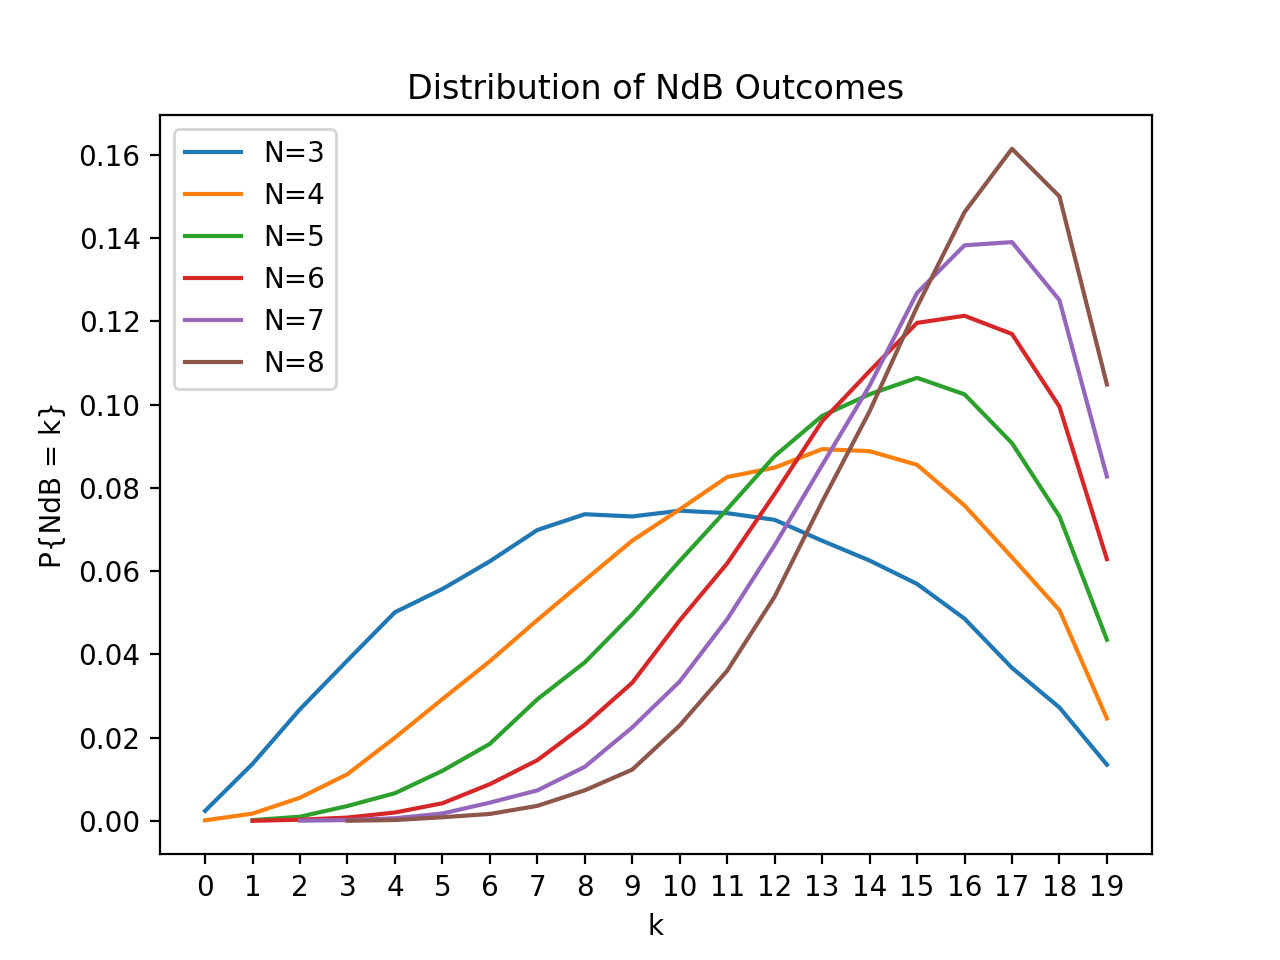
\includegraphics[scale=0.9]{outcome_distributions.png}
\caption{Distribution of the outcome of a $N\text{dB}$ check for various values of $N$.}
\end{figure}

\begin{figure}[ht]
\centering
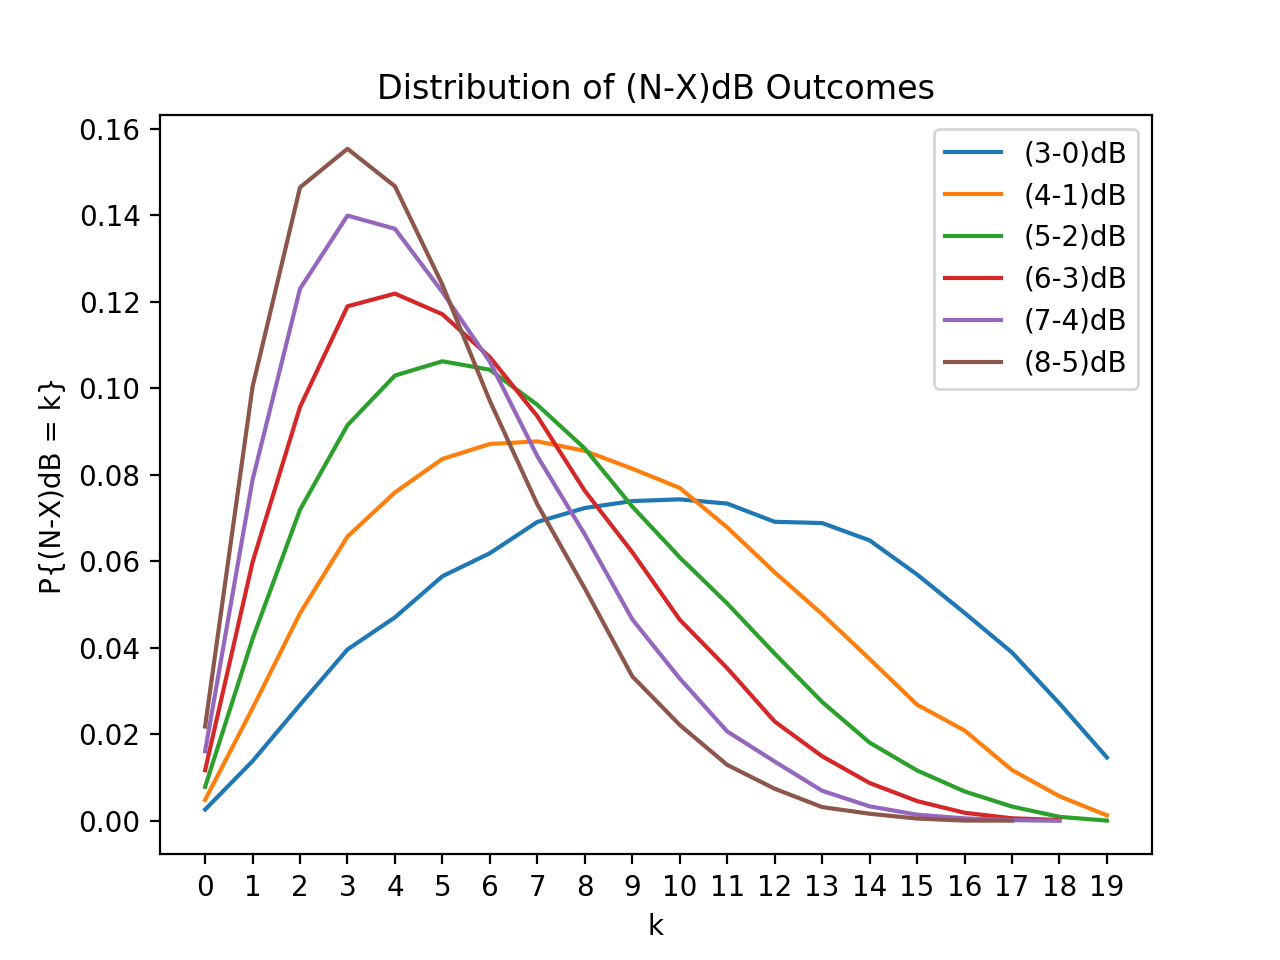
\includegraphics[scale=0.9]{discard_distributions.png}
\caption{Distribution of the outcome of a $(N-X)\text{dB}$ check for various values of $N$ and $X = N-3$.}
\end{figure}

\begin{figure}[ht]
\centering
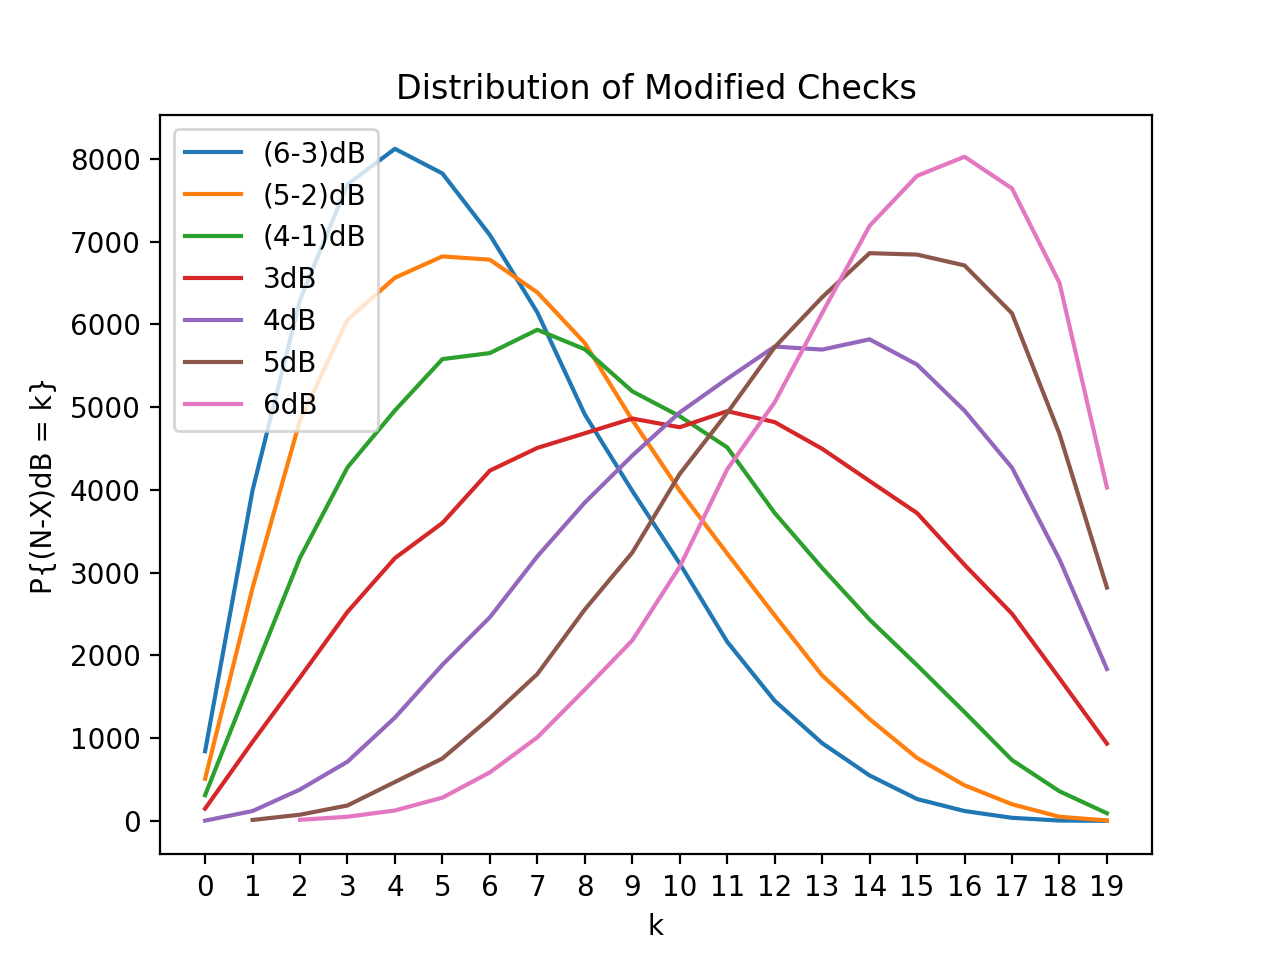
\includegraphics[scale=0.9]{modified_distributions.png}
\caption{Distribution of the outcome of modified $3$dB checks where the modifiers range from three negative to three positive.}
\end{figure}

\end{document}